\documentclass[10pt,letterpaper]{article}

\usepackage[T1]{fontenc}
\usepackage[utf8]{inputenc}
\usepackage{newtxtext,newtxmath}
\usepackage[letterpaper,margin=0.56in,top=0.48in,bottom=0.52in]{geometry}
\usepackage{microtype}
\usepackage{graphicx}
\usepackage{array}
\usepackage{booktabs}
\usepackage{tabularx}
\usepackage{enumitem}
\usepackage[table]{xcolor}
\usepackage{multicol}
\usepackage{fancyhdr}
\usepackage{titlesec}
\usepackage{needspace}
\usepackage[most]{tcolorbox}
\usepackage[hidelinks]{hyperref}

\graphicspath{{figures/}}

\definecolor{TitoInk}{HTML}{17201B}
\definecolor{TitoRed}{HTML}{B72831}
\definecolor{TitoRule}{HTML}{59605C}
\definecolor{TitoPale}{HTML}{F2F1EC}
\definecolor{TitoBlue}{HTML}{DDE8E6}
\definecolor{TitoDieBlue}{HTML}{2F6F8F}
\definecolor{TitoTan}{HTML}{D8C69F}

\setlength{\parindent}{0pt}
\setlength{\parskip}{3pt}
\setlength{\columnsep}{0.25in}
\setlength{\multicolsep}{6pt}
\setlist{nosep}
\renewcommand{\arraystretch}{1.12}

\pagestyle{fancy}
\fancyhf{}
\fancyhead[L]{\sffamily\scriptsize\color{TitoRule}TITO \textbullet\ PLAYBOOK}
\fancyhead[R]{\sffamily\scriptsize\color{TitoRule}GAME-TURNS 1--5}
\fancyfoot[C]{\sffamily\scriptsize TITO PLAYBOOK \textbullet\ \thepage}
\renewcommand{\headrulewidth}{0.35pt}
\renewcommand{\footrulewidth}{0pt}
\setlength{\headheight}{13pt}
\setlength{\footskip}{18pt}

\titleformat{\section}
  {\sffamily\bfseries\LARGE\color{TitoInk}}
  {}{0pt}{}
\titlespacing*{\section}{0pt}{7pt}{5pt}

\titleformat{\subsection}
  {\sffamily\bfseries\large\color{TitoInk}}
  {}{0pt}{}
\titlespacing*{\subsection}{0pt}{6pt}{3pt}

\newcommand{\rulesref}[1]{%
  {\sffamily\bfseries\color{TitoRed}[#1]}%
}

\newcommand{\phase}[1]{%
  \par\needspace{3\baselineskip}\vspace{4pt}%
  {\sffamily\bfseries\color{TitoInk}#1\par}%
  \vspace{1pt}{\color{TitoRule}\hrule height 0.35pt}\vspace{2pt}%
}

\newcommand{\turntitle}[3]{%
  \noindent
  \begin{minipage}[t]{0.16\textwidth}
    \vspace{0pt}
    {\sffamily\bfseries\fontsize{38}{38}\selectfont\color{TitoRed}#1\par}
    {\sffamily\bfseries\small GAME-TURN\par}
  \end{minipage}
  \hfill
  \begin{minipage}[t]{0.80\textwidth}
    \vspace{3pt}
    {\sffamily\bfseries\fontsize{23}{25}\selectfont\color{TitoInk}#2\par}
    \vspace{2pt}
    {\itshape #3\par}
  \end{minipage}
  \vspace{3pt}
  {\color{TitoInk}\hrule height 1pt}
  \vspace{5pt}
}

\newcommand{\die}[1]{%
  \tcbox[
    on line,
    colback=TitoDieBlue,
    colframe=TitoDieBlue,
    coltext=white,
    boxsep=0.2pt,
    left=3pt,right=3pt,top=1pt,bottom=1pt,
    arc=2pt
  ]{\sffamily\bfseries #1}%
}

\newcommand{\mapbadge}[1]{%
  \tikz[baseline=(badge.base)]{
    \node[
      circle,
      fill=TitoRed,
      text=white,
      font=\sffamily\bfseries\scriptsize,
      inner sep=1.2pt,
      minimum size=1.35em
    ] (badge) {#1};
  }%
}

\newtcolorbox{lessonbox}[1][]{
  enhanced,
  colback=TitoBlue!42,
  colframe=TitoRule,
  boxrule=0.45pt,
  arc=2pt,
  left=6pt,right=6pt,top=5pt,bottom=5pt,
  before skip=5pt,after skip=5pt,
  fonttitle=\sffamily\bfseries,
  coltitle=TitoInk,
  title={Rules in focus},
  #1
}

\newtcolorbox{commentarybox}[1][]{
  enhanced,
  colback=TitoPale,
  colframe=TitoPale,
  boxrule=0pt,
  arc=1pt,
  left=6pt,right=6pt,top=5pt,bottom=5pt,
  before skip=5pt,after skip=5pt,
  fonttitle=\sffamily\bfseries,
  coltitle=TitoInk,
  title={Play note},
  #1
}

\newcommand{\counterpic}[2][0.48in]{%
  \includegraphics[width=#1]{#2.pdf}%
}

\newcommand{\mapcaption}[1]{%
  \par\vspace{2pt}{\centering\sffamily\bfseries\scriptsize
  \color{TitoRule}#1\par}%
}

\newcommand{\turnledger}[5]{%
  \begin{tcolorbox}[
    colback=TitoPale,
    colframe=TitoRule,
    boxrule=0.4pt,
    arc=1pt,
    left=5pt,right=5pt,top=4pt,bottom=4pt,
    before skip=5pt,after skip=2pt
  ]
  \sffamily\footnotesize
  \begin{tabularx}{\linewidth}{@{}>{\bfseries}l X >{\bfseries}l X@{}}
    VP this turn & #1 & Running VP & #2 \\
    Partisans & #3 & Chetniks (Y/A/N) & #4 \\
    AGO expended & #5 & & \\
  \end{tabularx}
  \end{tcolorbox}
}

\begin{document}

\thispagestyle{empty}

\vspace*{0.25in}
{\sffamily\bfseries\fontsize{48}{48}\selectfont\color{TitoInk}TITO\par}
\vspace{2pt}
{\sffamily\bfseries\fontsize{25}{28}\selectfont\color{TitoRule}
  Playbook\par}
\vspace{7pt}
{\sffamily\bfseries\fontsize{18}{21}\selectfont\color{TitoRed}
  A Scripted Example of Play\par}
{\sffamily\large Game-Turns 1--5\par}

\vspace{10pt}
{\color{TitoInk}\hrule height 1.2pt}
\vspace{9pt}

\begin{center}
  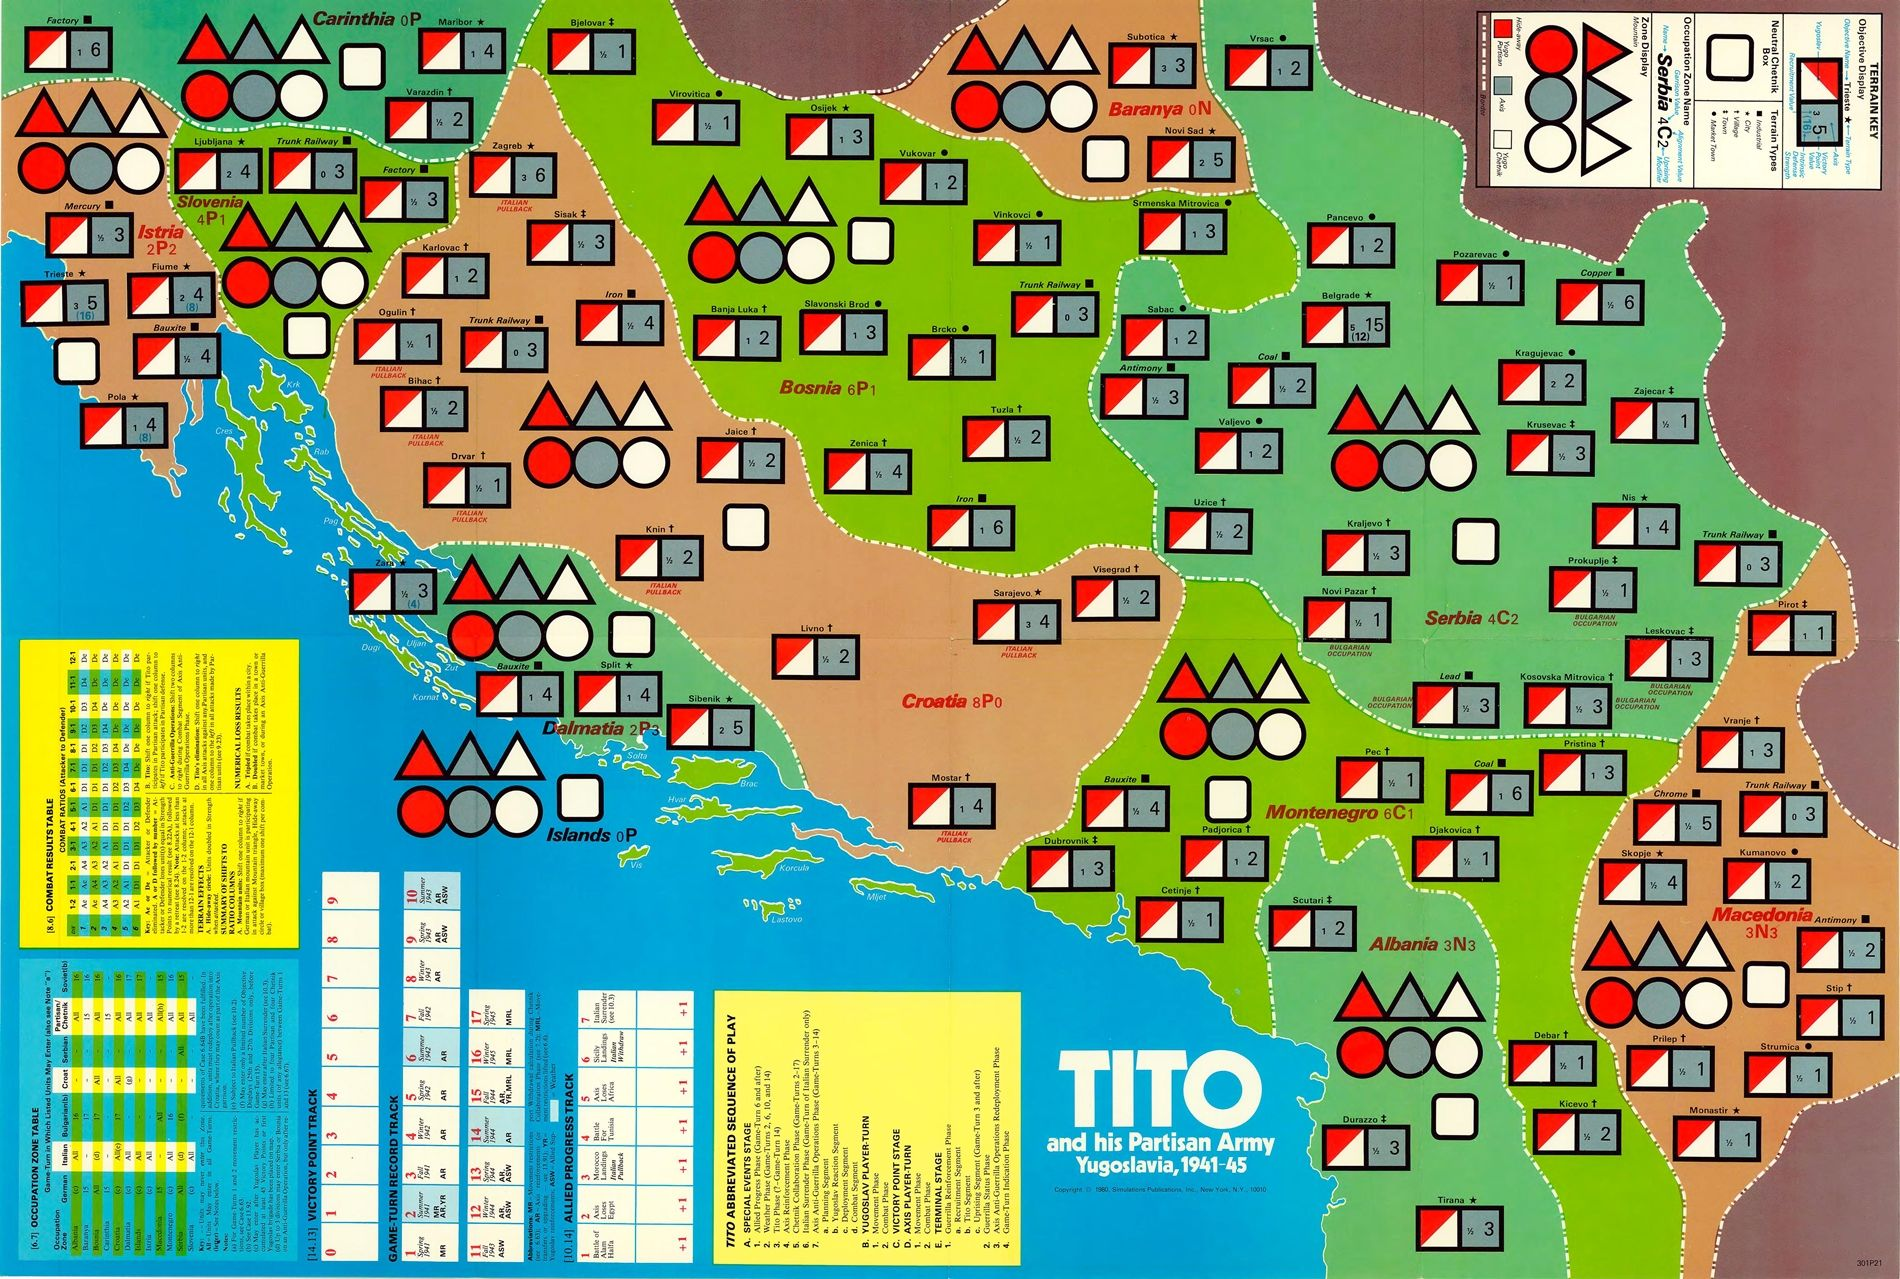
\includegraphics[width=0.96\linewidth,trim=0 105 0 0,clip]
    {../../Misc/Images/Tito/tito_map.jpg}
\end{center}

\vfill
\begin{minipage}[t]{0.57\textwidth}
  \small
  This playbook teaches the opening of \emph{Tito} by walking through a
  deliberately scripted game. The decisions are legal and plausible, but they
  are chosen to demonstrate systems rather than provide perfect strategy.
  Follow the stated setup and use the printed die rolls to reproduce the
  example at the table.
\end{minipage}
\hfill
\begin{minipage}[t]{0.37\textwidth}
  \raggedleft
  {\sffamily\bfseries Presentation by Daniel J. Berger\par}
  {\sffamily Version 0.1\par}
  {\sffamily \today\par}
\end{minipage}

\clearpage

\section{How to Use This Playbook}

\begin{multicols}{2}
\small
The example follows the complete Sequence of Play, but compresses phases in
which no choice or game-state change occurs. Every prescribed die roll is
shown in a red box. Rules citations point to the restored rulebook.

The map illustrations are snapshots, not stack inventories. Numbered callouts
match the accompanying prose; exact stacks are stated in the text and in each
turn ledger. Counters are not drawn to scale.

\begin{lessonbox}
\begin{itemize}[leftmargin=1.2em,itemsep=2pt]
  \item Game-Turn 1: movement, objectives, combat, retreat, and recruitment.
  \item Game-Turn 2: drought, Chetnik collaboration, and Tito.
  \item Game-Turn 3: Anti-Guerrilla Operations and uprisings.
  \item Game-Turn 4: winter, brigade formation, and expanded Axis movement.
  \item Game-Turn 5: locating Tito and an elimination attempt.
\end{itemize}
\end{lessonbox}

\columnbreak

\subsection{Contents}

\begin{tabularx}{\linewidth}{@{}Xr@{}}
  Preparing the Game & 3 \\
  Game-Turn 1: Testing the Occupation & 4 \\
  Game-Turn 2: Tito Enters the War & 5 \\
  Game-Turn 3: The War Spreads & 6 \\
  Game-Turn 4: Winter and Escalation & 8 \\
  Game-Turn 5: The Hunt for Tito & 9 \\
  After Five Turns & 10 \\
\end{tabularx}

\subsection{Conventions}

\begin{tabularx}{\linewidth}{@{}>{\bfseries}l X@{}}
  P & Partisan \\
  C & Chetnik \\
  Y/A/N & pro-Yugoslav, pro-Axis, neutral \\
  SP & Combat Strength Points \\
  AGO & Anti-Guerrilla Operation \\
  GT & Game-Turn \\
\end{tabularx}

\begin{commentarybox}
This tutorial uses the original restored rules. It does not employ the
unverified online addenda.
\end{commentarybox}
\end{multicols}

\vfill
\begin{center}
  \counterpic[0.62in]{german-infantry-front}\hspace{0.13in}
  \counterpic[0.62in]{chetnik-group}\hspace{0.13in}
  \counterpic[0.62in]{tito-unidentified}\hspace{0.13in}
  \counterpic[0.62in]{partisan-group}\hspace{0.13in}
  \counterpic[0.62in]{partisan-brigade}
\end{center}

\clearpage
\section{Preparing the Game}

\begin{lessonbox}
Set up every unit listed in \rulesref{15.1--15.2}. The choices below specify
only the locations that matter to the tutorial. Units not named individually
may occupy any legal Objective Display in their assigned Zone; keep
\textbf{Pančevo} and \textbf{Cetinje} free of Axis units.
\end{lessonbox}

\begin{multicols}{2}
\small
\subsection{Key Axis Placements}

\rowcolors{2}{TitoBlue!42}{white}
\begin{tabularx}{\linewidth}{@{}>{\bfseries}l X@{}}
  \rowcolor{TitoInk!15}
  Unit & Objective Display \\
  German 704 & Belgrade \\
  German 714 & Kragujevac \\
  German 717 & Niš \\
  German 718 & Sarajevo \\
  Serbian 1--5 & Belgrade \\
  Italian Bergamo & Zagreb \\
  Italian Sassari & Karlovac \\
  Italian Macerata & Padgorica \\
\end{tabularx}
\rowcolors{2}{}{}

Place the remaining Italians throughout their assigned Zones, but leave
Cetinje empty. Place the Bulgarian 14th, 22nd, and 24th Divisions in Skopje,
Prilep, and Monastir respectively.

\subsection{Yugoslav Placements}

Place five Chetnik groups in the Serbia Chetnik Hide-away and two in the
Montenegro Chetnik Hide-away. All seven begin pro-Yugoslav.

\subsection{AGO Limit}

For this example, the Axis Player draws the Soviet counter with
\textbf{8 AGO} on its reverse. Keep it concealed as normal
\rulesref{15.31--15.32}. The example will expend three operations by the end
of Game-Turn 5.

\columnbreak

\subsection{Why This Setup?}

The starting deployments preserve the historical spheres of influence while
creating two safe Yugoslav probes:

\begin{itemize}[leftmargin=1.2em,itemsep=2pt]
  \item Pančevo offers the Chetniks a useful Recruitment Value of 1 and a
    Victory Point Value of 2.
  \item Cetinje offers a smaller but initially unopposed foothold.
  \item The German divisions remain close enough to demonstrate the Axis
    three-Zone movement allowance and a mandatory Objective combat.
  \item Croatia and Bosnia remain under-garrisoned, setting up the first
    uprising checks on Game-Turn 3.
\end{itemize}

\begin{commentarybox}
The original setup rules assign units to Zones, not to particular Objective
Displays. This freedom is intentional: two legal games can begin with quite
different local situations.
\end{commentarybox}

\subsection{Starting Tracks}

\begin{tabularx}{\linewidth}{@{}>{\bfseries}l X@{}}
  Game-Turn & 1 \\
  Yugoslav VP & 0 \\
  Allied Progress & Not yet begun \\
  Weather & Normal \\
  Tito & Not yet on map \\
  Partisan strength & 0 groups \\
  Chetnik strength & 7 pro-Yugoslav groups \\
\end{tabularx}
\end{multicols}

\vfill
\begin{center}
  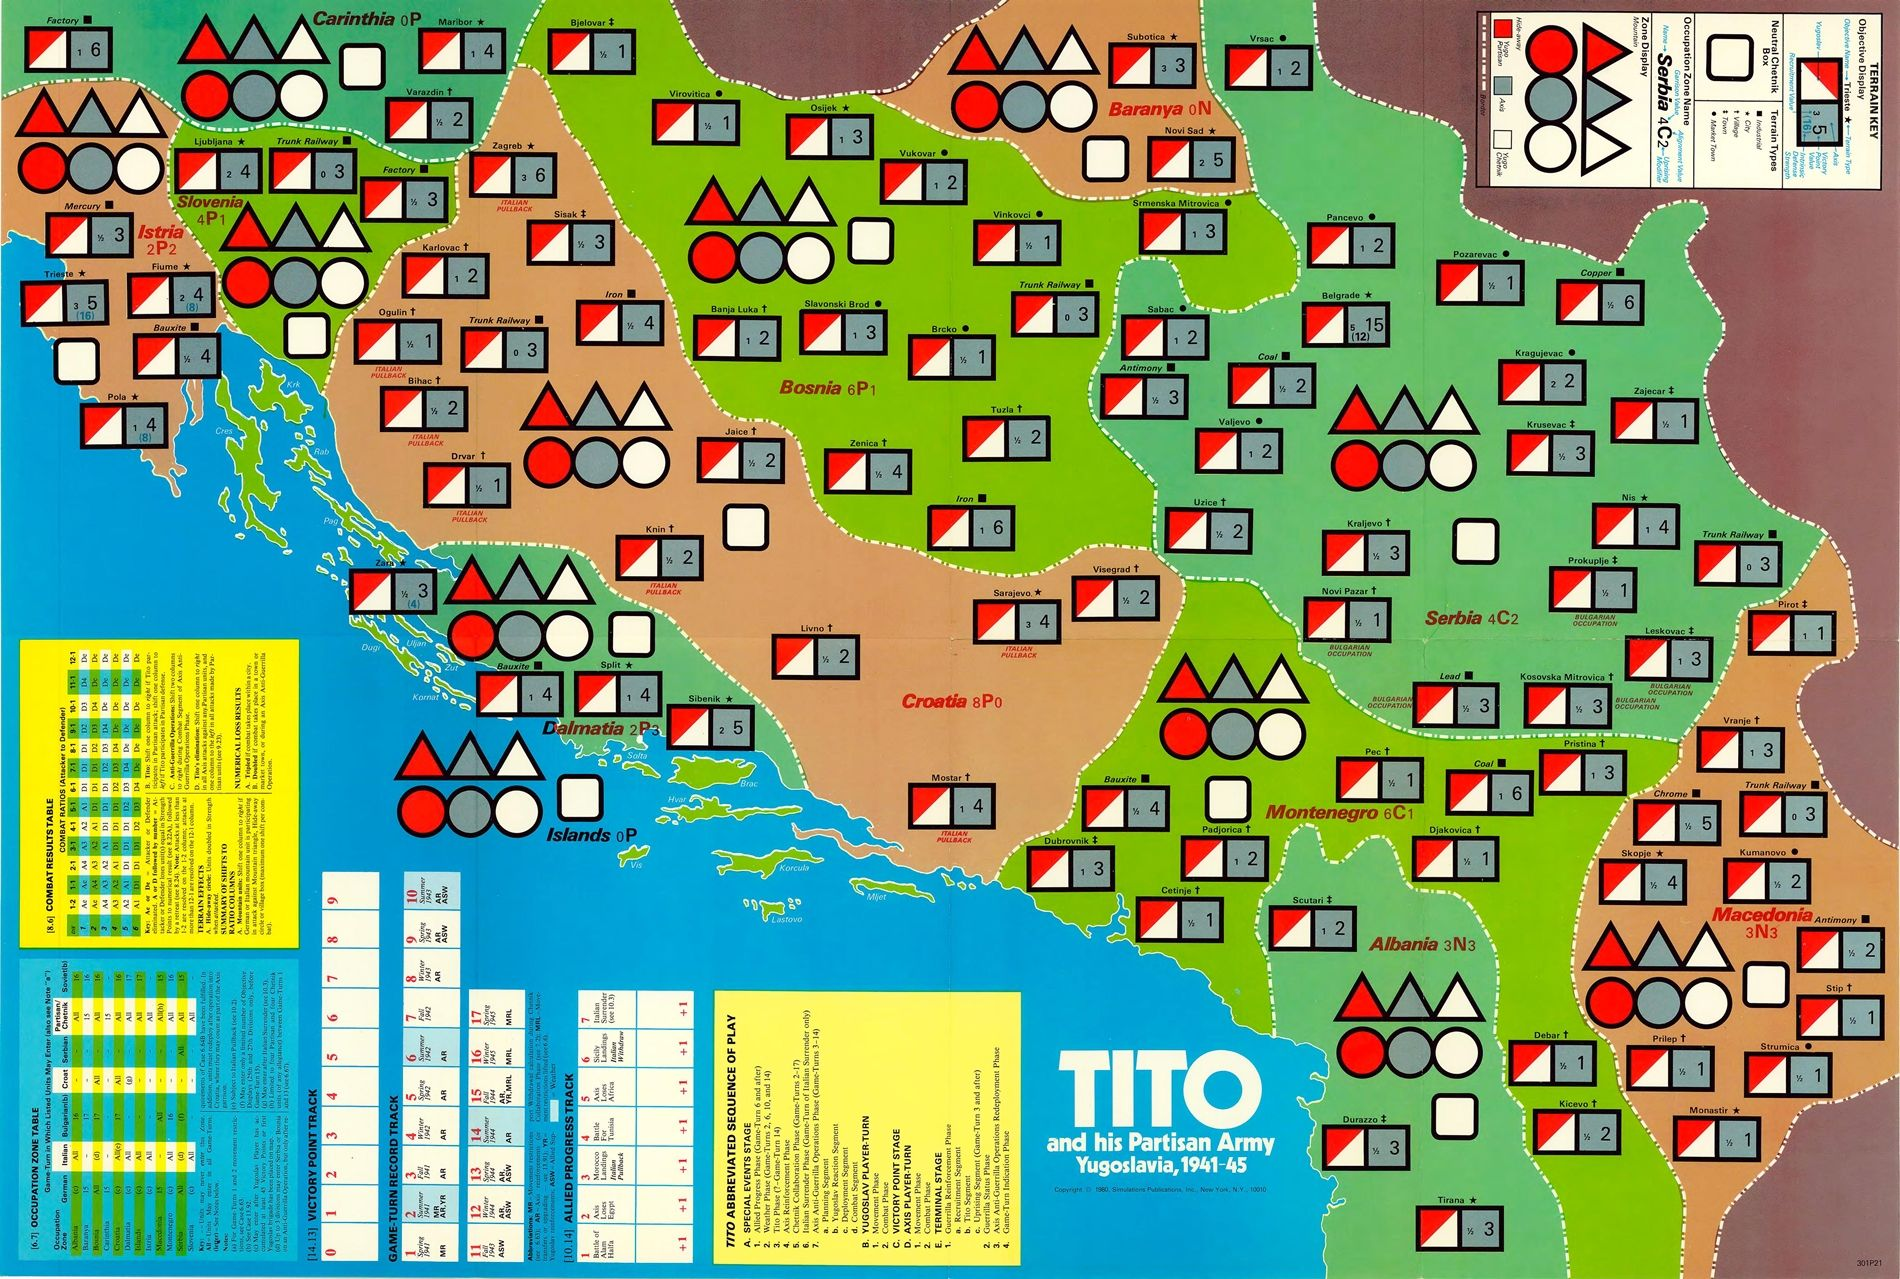
\includegraphics[width=0.67\linewidth,trim=70 120 40 70,clip]
    {../../Misc/Images/Tito/tito_map.jpg}
\end{center}

\begin{center}
\scriptsize\itshape
The full map before counters are placed. The tutorial’s opening action is
concentrated in Serbia and Montenegro; the conflict expands west on Turn 3.
\end{center}

\playbookbreak
\turntitle{1}{Testing the Occupation}
  {The Chetniks probe two undefended objectives; the Axis answers at Pančevo.}

\begin{lessonbox}
\rulesref{4.1} Game-Turn 1 begins with the Yugoslav Player-Turn, so the entire
Special Events Stage is skipped. Both sides must remain within their starting
Zones on Game-Turns 1 and 2 \rulesref{6.63, 15.4}.
\end{lessonbox}

\begin{center}
\begin{minipage}[t]{0.62\linewidth}
  \centering
  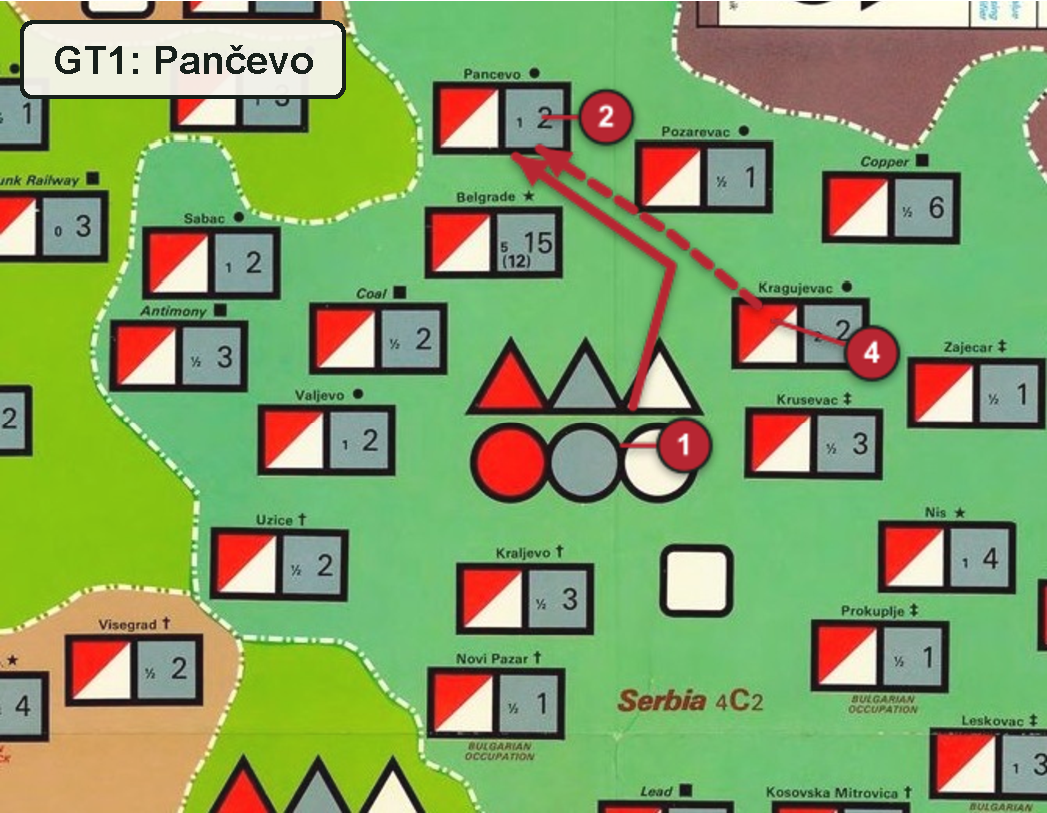
\includegraphics[width=\linewidth]{playbook-turn-1-map.pdf}
  \mapcaption{Serbia: the Pančevo probe and German reply}
\end{minipage}
\hfill
\begin{minipage}[t]{0.34\linewidth}
  \centering
  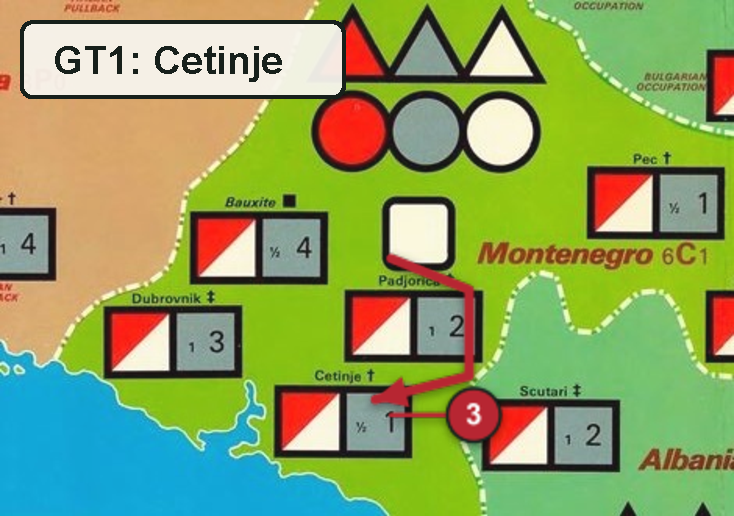
\includegraphics[width=\linewidth]{playbook-turn-1-south-map.pdf}
  \mapcaption{Montenegro: the unopposed move to Peć}
\end{minipage}
\end{center}

\begin{multicols}{2}
\small
\phase{B. Yugoslav Player-Turn}

\textbf{Movement.} From the Serbia Hide-away~\mapbadge{1}, move three Chetnik
groups to Pančevo~\mapbadge{2} and two to the Chetnik Mountain triangle. From
the Montenegro Hide-away, move both groups to Peć~\mapbadge{3}. All
movement is within the units' starting Zones.

\textbf{Combat.} The Axis boxes of Pančevo and Peć are empty, so there is
no corresponding enemy stack and no combat \rulesref{8.11}.

\phase{C. Victory Point Stage}

Pančevo is worth 2 VP and Peć 1 VP. The Yugoslav Player gains
\textbf{3 VP}. The two groups in the Serbia Mountain yield no Mountain VP:
$2 \div 4$, rounded down, is zero \rulesref{14.2B}.

\phase{D. Axis Player-Turn}

German 714 moves from Kragujevac to the Axis box at Pančevo~\mapbadge{4}.
Opposing units now occupy corresponding Objective boxes, so combat is
mandatory.

\begin{commentarybox}[title={Combat calculation}]
German 714 attacks with 12 SP against 3 Chetnik SP: \textbf{4:1}. The Axis
Player rolls \die{3}, producing \textbf{D1}. Pančevo is a market town, so the
numbered result is doubled to \textbf{D2} \rulesref{8.32B}. Two groups are
removed and the survivor retreats to the Serbia Chetnik Hide-away
\rulesref{8.24A}.
\end{commentarybox}

\columnbreak

\phase{E. Terminal Stage}

\textbf{Recruitment.} The two Chetnik groups at Peć occupy an Objective
with a Recruitment Value of one-half. The Yugoslav Player rolls \die{4}, so
$4 \times \tfrac{1}{2}=2$ groups. This does not exceed the two occupying
Yugoslav SP, so two new Chetnik groups are placed at Peć \rulesref{7.44A}.
Peć now contains four.

The two Chetnik groups in the Serbia Mountain create none:
$2 \div 4=0$ after fractions are dropped \rulesref{7.45}.

There is no Tito Segment, no Uprising Segment before Game-Turn 3, and neither
guerrilla type has reached brigade strength. Advance the Game-Turn marker.

\subsection{What the Turn Demonstrated}

\begin{itemize}[leftmargin=1.2em,itemsep=2pt]
  \item A unit may move freely among locations within its Zone.
  \item Combat in corresponding Objective boxes is mandatory.
  \item Terrain modifies a numbered combat result, not the combat ratio.
  \item Yugoslav retreats go to the appropriate Hide-away.
  \item Objective recruitment is limited by occupying Yugoslav SP.
\end{itemize}
\end{multicols}

\turnledger{+3}{3}{None}{7 / 0 / 0}{0 of 8}

\playbookbreak
\turntitle{2}{Tito Enters the War}
  {Weather, collaboration, and predetermined Partisan reinforcements transform
  the map.}

\iftextonly
  \begin{multicols}{2}
  \small
\else
  \noindent
  \begin{minipage}[t]{0.49\linewidth}
  \vspace{0pt}
  \centering
  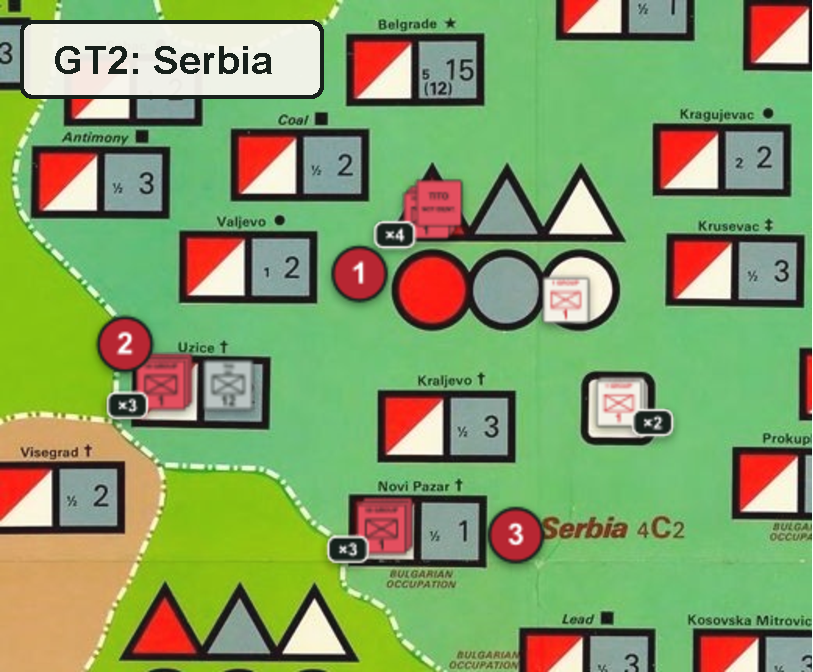
\includegraphics[width=\linewidth]{playbook-turn-2-map.pdf}
  \mapcaption{Serbia: Tito and ten groups divide}

  \raggedright\small
\fi
\phase{A. Special Events Stage}

\textbf{Weather.} The Yugoslav Player rolls \die{2}; drought is in effect for
Game-Turns 2--5 \rulesref{11.21--11.23}. Drought halves recruitment in market
towns, but does not affect towns or Mountains.

\textbf{Axis reinforcements.} Place German 342 at Kragujevac (Serbia), German
125 at Tuzla (Bosnia), and the Croat Guard regiment and 1st--3rd Ustaša
brigades at Zagreb (Croatia) \rulesref{13.91}.

\smallskip
\textbf{Chetnik collaboration.} Roll once for each occupied Chetnik location
\rulesref{7.21, 7.23A}:

\begin{tabularx}{\linewidth}{@{}Xccc@{}}
  \toprule
  Stack & Roll & Modifier & Result \\
  \midrule
  Serbia Mountain (2) & \die{2} & +1 & Neutral \\
  Serbia Hide-away (1) & \die{4} & +1 & pro-Yugoslav \\
  Peć (4) & \die{1} & +1 & pro-Axis \\
  \bottomrule
\end{tabularx}

Move the neutral stack to Serbia's Neutral Chetnik box and the pro-Axis stack
to Montenegro's Axis Mountain \rulesref{7.24}.

\phase{B. Yugoslav Player-Turn}

At the beginning of Movement, place the predetermined reinforcements
\rulesref{7.41, 13.92}. There are 17 groups: 10 plus Tito in Serbia, 4 in
Slovenia, and 3 in Montenegro. All groups are P1 and are placed in their
respective Partisan Hide-away circles. Because Game-Turn 2 still has the
starting-Zone restriction, move them as follows:

\smallskip
\begin{itemize}[leftmargin=1.2em,itemsep=1.5pt]
  \item Serbia: three groups to Užice~\mapbadge{2}, three to Novi Pazar
    ~\mapbadge{3}, and four plus Tito to the Partisan Mountain~\mapbadge{1}.
  \item Slovenia: all four groups to the Partisan Mountain~\mapbadge{4}.
  \item Montenegro: all three groups to Peć~\mapbadge{5}.
\end{itemize}

\begin{commentarybox}
Tito is a unit for movement and reaction purposes, but has no Combat Strength.
His immediate value is organizational: he generates Partisan groups and must
be present when the first Partisan brigade is formed.
\end{commentarybox}
\iftextonly
\else
  \end{minipage}
  \hfill
  \begin{minipage}[t]{0.49\linewidth}
  \vspace{0pt}
  \centering
  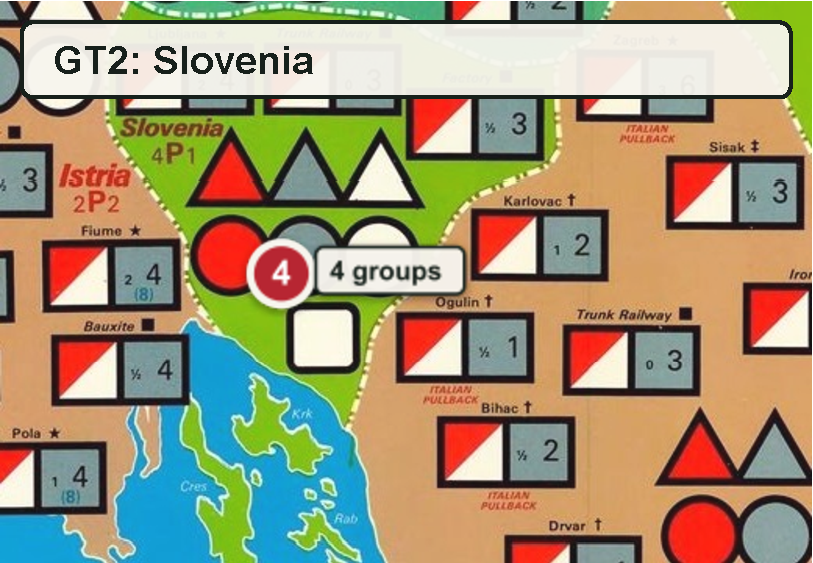
\includegraphics[width=0.78\linewidth]{playbook-turn-2-slovenia-map.pdf}
  \mapcaption{Slovenia}

  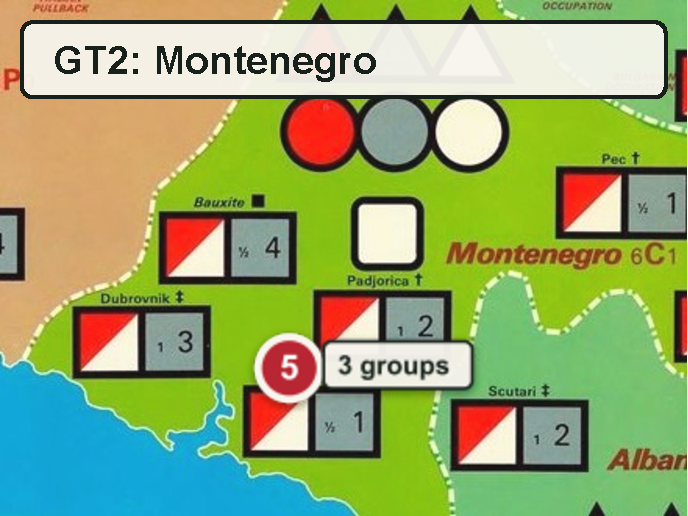
\includegraphics[width=0.78\linewidth]{playbook-turn-2-south-map.pdf}
  \mapcaption{Montenegro}

  \raggedright\small
\fi
\phase{C. Victory Point Stage}

Užice, Novi Pazar, and Peć yield 4 VP. The Serbia and Slovenia Mountains
each contain 4 Partisan SP and yield 1 VP. Gain \textbf{6 VP}; the running
total is \textbf{9}.

\phase{D. Axis Player-Turn}

\textbf{Movement.} German 704 moves from Belgrade to the Axis box at Užice.
Italian Macerata moves from Padjorica to the Axis box at Peć, while Italian Re
moves from Cetinje to the newly vacated Axis box at Padjorica. All three units
remain within their starting Zones \rulesref{6.16, 6.63}.

\smallskip
\textbf{Combat.} German 704 attacks the three groups in Užice. At 12:3 the
ratio is 4:1; a \die{3} produces D1, doubled to D2 for the town. Two groups
are removed and one retreats to the Serbia Partisan Hide-away.

Italian Macerata attacks Peć at 6:3, or 2:1. A \die{5} produces D1,
doubled to D2. Again, two groups are removed and the survivor retreats.

\phase{E. Terminal Stage}

\textbf{Recruitment rolls:}

\begin{itemize}[leftmargin=1.2em,itemsep=1.5pt]
  \item Novi Pazar: \dr{4} times one-half creates 2 groups.
  \item Serbia Mountain: $4 \div 4$ creates 1 group.
  \item Slovenia Mountain: $4 \div 4$ creates 1 group.
  \item Tito in Serbia creates 1 group \rulesref{7.46C}.
\end{itemize}

\smallskip
The Partisans finish with $17-4+5=\textbf{18 groups}$. There are still no
uprisings and no organization upgrades.
\iftextonly
  \end{multicols}
\else
  \end{minipage}
\fi

\turnledger{+6}{9}{18 groups}{1 / 4 / 2}{0 of 8}

\clearpage
\turntitle{3}{The War Spreads}
  {The first Anti-Guerrilla Operation drives Tito west; uprisings bring the
  Partisans to brigade strength.}

\begin{lessonbox}
Game-Turn 3 activates two major systems: Axis Anti-Guerrilla Operations
\rulesref{8.4} and the Uprising Segment \rulesref{7.47, 7.5}. The
starting-Zone restriction has also expired.
\end{lessonbox}

\begin{center}
\begin{minipage}[t]{0.48\linewidth}
  \centering
  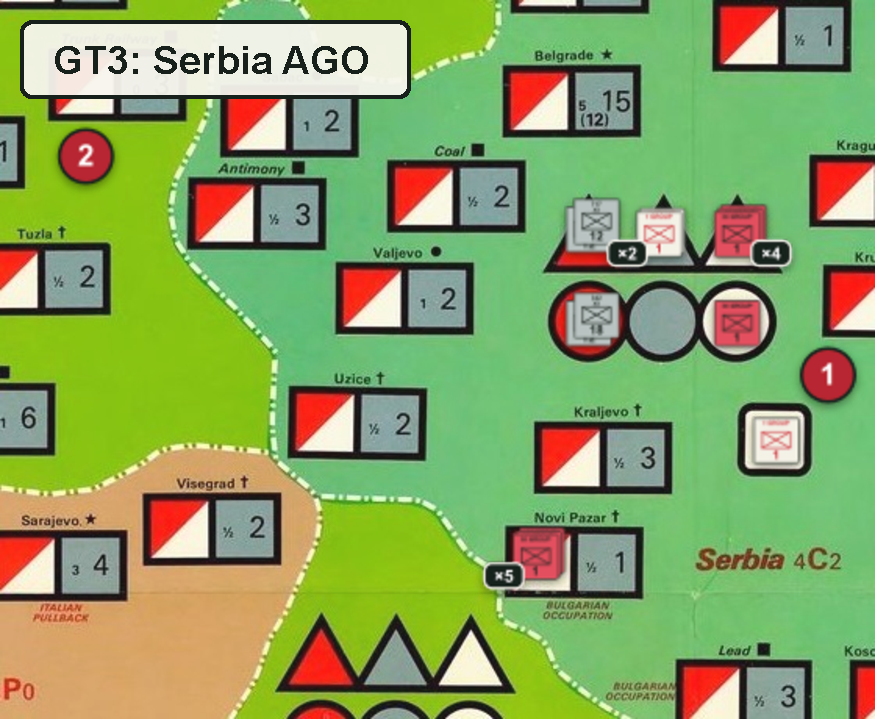
\includegraphics[width=\linewidth]{playbook-turn-3-map.pdf}
  \mapcaption{Serbia: AGO deployment and the reaction route west}
\end{minipage}
\hfill
\begin{minipage}[t]{0.48\linewidth}
  \centering
  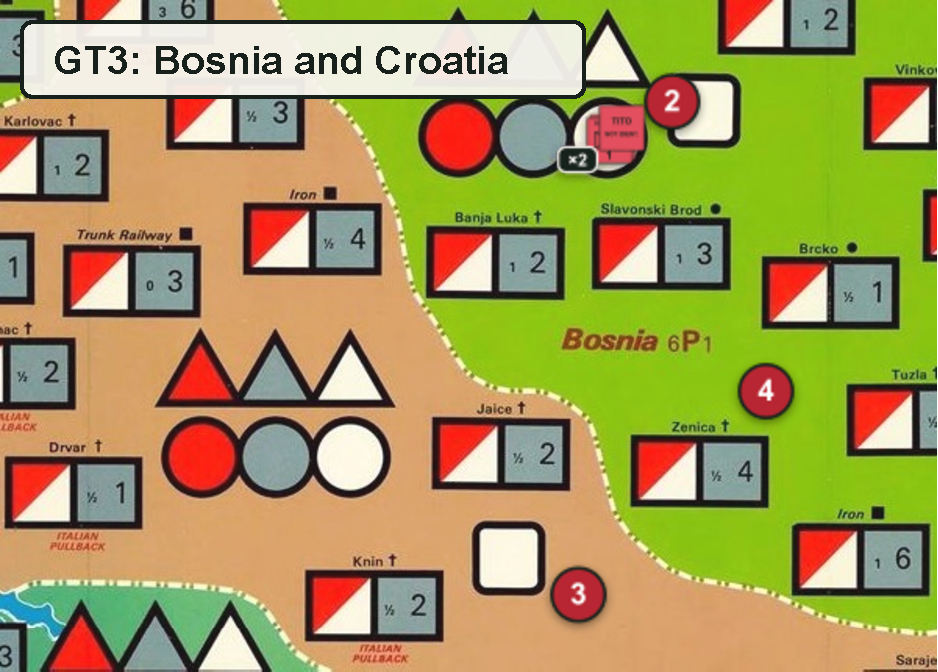
\includegraphics[width=\linewidth]{playbook-turn-3-west-map.pdf}
  \mapcaption{Bosnia and Croatia: Tito's refuge and uprising checks}
\end{minipage}
\end{center}

\begin{multicols}{2}
\small
\phase{A. Reinforcement and Collaboration}

Place German 113 in Bosnia and the 4th and 5th Ustaša brigades in Croatia.
Transfer German 125 as scheduled \rulesref{13.91}.

Resolve collaboration:

\begin{tabularx}{\linewidth}{@{}Xccc@{}}
  \toprule
  Stack & Roll & Mod. & Result \\
  \midrule
  Serbia neutral (2) & \die{5} & 0 & pro-Yugoslav \\
  Serbia pro-Yugoslav (1) & \die{3} & +1 & Neutral \\
  Montenegro pro-Axis (4) & \die{5} & $-1$ & Neutral \\
  \bottomrule
\end{tabularx}

The Axis Player now has no Chetnik groups under control, but this calm will not
last.

\phase{A. Axis Anti-Guerrilla Operations Phase}

\textbf{Planning.} The Axis declares one operation and secretly records
\mbox{\emph{Serbia}~\mapbadge{1}}. German 704, 714, 717, and 342 are selected; each
could reach Serbia in a normal Movement Phase and the total is below seven
division equivalents \rulesref{8.41--8.42}.

\textbf{Reaction.} The Yugoslav Player rolls \die{3}. Tito and two Partisan
groups leave the Serbia Mountain for the Bosnia Partisan
Hide-away~\mapbadge{2}. Tito counts as one of the three reacting units. Four groups
remain in the Serbia Mountain.

\columnbreak

\textbf{Deployment and combat.} Put 714 and 717 in the Axis Mountain and 704
and 342 in the Axis Hide-away:

\begin{itemize}[leftmargin=1.2em,itemsep=2pt]
  \item \textbf{Mountain:} 24 SP attacks 4 SP at 6:1. The AGO adjustment moves
    this to 8:1. A \die{1} produces D1, doubled to D2. Two groups are lost and
    two retreat to the Bosnia Partisan Hide-away.
  \item \textbf{Hide-away:} 30 SP attacks the lone group that retreated from
    Užice. Its defensive strength is doubled to 2, yielding 15:1, capped at
    12:1. A \die{1} produces De and eliminates it.
\end{itemize}

The four German divisions are removed pending redeployment
\rulesref{8.47}. The Yugoslav Player has lost three groups, but the reaction
saved Tito and gave the survivors a common refuge in Bosnia.

\begin{commentarybox}
An AGO changes the ratio by two columns, doubles numbered results, and sends
retreating Yugoslav units to an adjacent Zone. Axis units are never forced to
retreat during the operation \rulesref{8.46}.
\end{commentarybox}

\subsection{Situation After the Operation}

\begin{tabularx}{\linewidth}{@{}>{\bfseries}l X@{}}
  Bosnia Hide-away & Tito and 4 Partisan groups \\
  Serbia & 5 groups at Novi Pazar; no Partisans in the Zone Display \\
  Slovenia Mountain & 5 Partisan groups \\
  Montenegro Hide-away & 1 Partisan group \\
  Partisan total & 15 groups \\
\end{tabularx}
\end{multicols}

\clearpage
\turntitle{3}{From Groups to Brigades}
  {Recruitment and two under-garrisoned Zones fill the Partisan counter pool.}

\begin{multicols}{2}
\small
\phase{B. Yugoslav Player-Turn}

Move Tito and all four Bosnia groups from the Hide-away to the Partisan
Mountain, then send one group to Tuzla. Three groups remain with Tito. Keep the
five-group stack at Novi Pazar and the five groups in the Slovenia Mountain.
Move the lone Montenegro group back to Cetinje.

\phase{C. Victory Point Stage}

Novi Pazar, Tuzla, and Cetinje yield 4 VP. The Slovenia Mountain yields 1 VP
for its 5 SP. The Bosnia Mountain has only 3 SP and yields none. Gain
\textbf{5 VP}; the running total becomes \textbf{14}.

\phase{D. Axis Player-Turn}

The Axis emphasizes garrison duty and initiates no Objective combat. Units
used in the Serbia AGO remain off map until the Redeployment Phase, but may
count toward Serbia's garrison because that was the target Zone
\rulesref{7.54}.

\phase{E. Recruitment and Tito Segments}

The Partisans begin the Terminal Stage with 15 groups:

\begin{tabularx}{\linewidth}{@{}Xr@{}}
  \toprule
  Source & Groups \\
  \midrule
  Novi Pazar: \die{6} $\times$ one-half, cap 5 & 3 \\
  Slovenia Mountain: $5 \div 4$ & 1 \\
  Tuzla: \die{6} $\times$ one-half, cap 1 & 1 \\
  Cetinje: \die{4} $\times$ one-half, cap 1 & 1 \\
  Tito in Bosnia & 2 \\
  \midrule
  Total before uprisings & 23 \\
  \bottomrule
\end{tabularx}

\columnbreak

\phase{E. Uprising Segment}

\textbf{Croatia~\mapbadge{3}.} Two Italian divisions, the Croat Guard regiment,
and five Ustaša brigades equal $4\tfrac{5}{6}$ divisions. Drop the fraction
when calculating the shortfall: Croatia is four divisions below its Garrison
Value of 8. The uprising roll is \die{1}; with a modifier of 0, the modified
result is 1. Four short divisions times 1 creates \textbf{4 groups}. An
alignment roll of \die{4} is even, so all are Partisan in this P-aligned Zone.

\textbf{Bosnia~\mapbadge{4}.} German 718 and 113 provide two divisions against
a Garrison Value of 6. A \die{2}, less Bosnia's modifier of 1, gives a modified
result of 1. Four more Partisan groups would be created after an even alignment
roll of \die{2}, but only three Partisan group counters remain. Place those
three in the Bosnia Partisan Hide-away \rulesref{7.53, 7.68}.

The Partisans now have all \textbf{30 group counters} on the map and have
achieved brigade strength \rulesref{7.62A}.

\phase{E. Guerrilla Status Phase}

The first brigade must be created where Tito is located. Five groups occupy
the Bosnia Mountain with Tito: three moved there and two arrived in the Tito
Segment. Replace three with the 31st Partisan Brigade. Two groups remain with
Tito \rulesref{7.63, 7.67}.

\begin{commentarybox}[title={The important trigger}]
The first Partisan brigade has appeared. Beginning next Game-Turn, German
movement expands into the Italian sphere, the Bulgarian 25th and 27th
Divisions become available, and the Axis may attempt to identify Tito
\rulesref{6.64, 9.41, 13.91D}.
\end{commentarybox}
\end{multicols}

\turnledger{+5}{14}{27 groups + 1 brigade}{2 / 0 / 5}{1 of 8}

\vspace{0.7em}
\begin{multicols}{2}
\small
\subsection{Checkpoint Before Game-Turn 4}

\begin{tabularx}{\linewidth}{@{}>{\bfseries}l X@{}}
  Bosnia Mountain & Tito, 31st Brigade, 2 groups \\
  Bosnia Hide-away & 3 groups \\
  Tuzla & 2 groups \\
  Croatia Hide-away & 4 groups \\
  Slovenia Mountain & 6 groups \\
  Novi Pazar & 8 groups \\
  Cetinje & 2 groups \\
\end{tabularx}

Redeploy the four German AGO divisions in Serbia. The first-brigade trigger is
now permanent even if Partisan strength later falls below 30 group
equivalents.

\columnbreak

\subsection{What the Turn Demonstrated}

\begin{itemize}[leftmargin=1.2em,itemsep=3pt]
  \item An AGO is planned before reaction, so the Axis commits units without
    knowing exactly which guerrillas will remain.
  \item Reaction can preserve Tito and concentrate scattered survivors in an
    adjacent Zone.
  \item AGO participants still count toward the target Zone's garrison while
    awaiting redeployment.
  \item Objective recruitment, Tito, and uprisings all resolve before the
    Guerrilla Status Phase.
  \item Counter availability is a hard limit: excess uprising reinforcements
    are lost.
\end{itemize}

\begin{commentarybox}[title={A real decision}]
The first brigade need not be the 31st, and the Yugoslav Player could leave
all five Bosnia Mountain groups unorganized. Creating it now is stronger and
activates several Axis responses; delaying it conceals Tito for longer.
\end{commentarybox}
\end{multicols}

\playbookbreak
\turntitle{4}{Winter and Escalation}
  {The first brigade unlocks a wider Axis response, while winter suppresses
  Mountain recruitment.}

\begin{center}
\begin{minipage}[t]{0.56\linewidth}
  \centering
  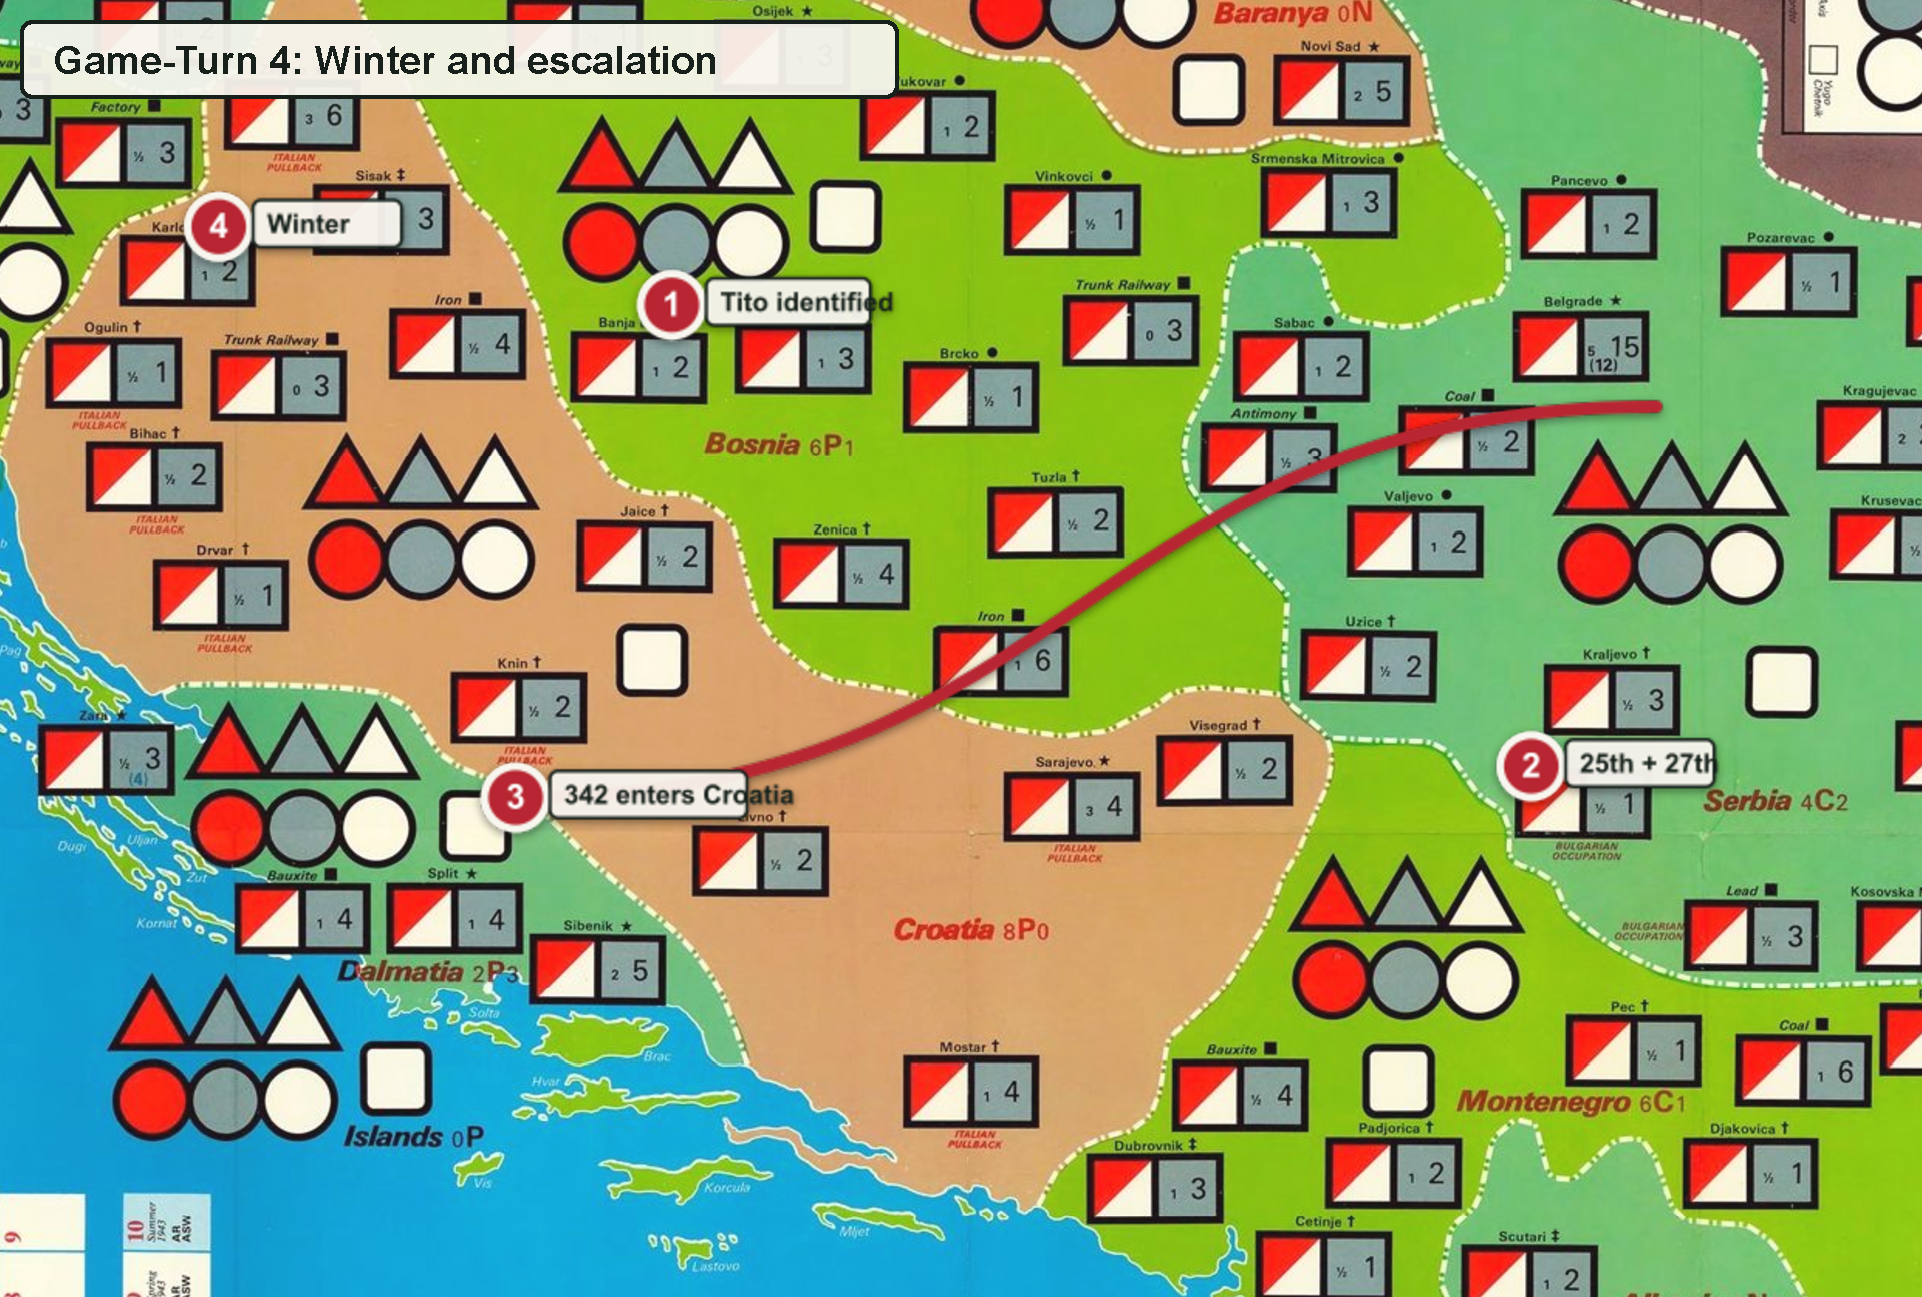
\includegraphics[height=2.42in,width=\linewidth,keepaspectratio]
    {playbook-turn-4-map.pdf}
  \mapcaption{West: Tito is identified and German 342 enters Croatia}
\end{minipage}
\hfill
\begin{minipage}[t]{0.40\linewidth}
  \centering
  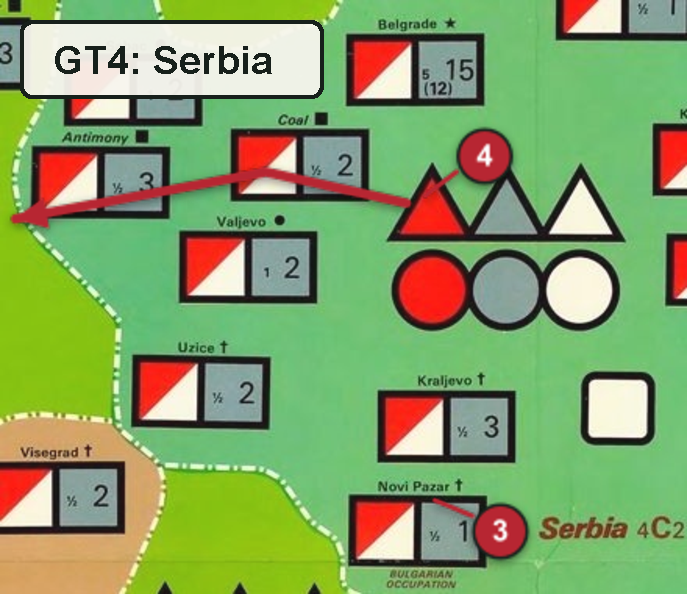
\includegraphics[height=2.42in,width=\linewidth,keepaspectratio]
    {playbook-turn-4-east-map.pdf}
  \mapcaption{Serbia: Bulgarian 25th and 27th enter}
\end{minipage}
\end{center}

\begin{multicols}{2}
\small
\phase{A. Special Events Stage}

\textbf{Winter.} Game-Turn 4 is automatically Winter
\rulesref{11.1}. Recruitment in villages and Mountains will be halved.

\textbf{Tito Phase.} Because the first Partisan brigade appeared last turn,
the Axis may attempt to identify Tito. A \die{6} succeeds; flip Tito to his
identified side~\mapbadge{1} \rulesref{9.41}.

\textbf{Axis reinforcements.} Transfer German 113 from Zenica. In Bosnia,
place six new Croat brigades at Zenica, including mountain brigades 1--4;
place the other four at Zagreb (Croatia). The brigade trigger also releases
Bulgarian 25 and 27; place them at Prokuplje and Leskovac, respectively, in
Serbia~\mapbadge{3} \rulesref{13.91D}.

\textbf{Collaboration.}

\begin{tabularx}{\linewidth}{@{}Xccc@{}}
  \toprule
  Stack & Roll & Mod. & Result \\
  \midrule
  Serbia pro-Yugoslav (2) & \die{3} & +1 & Neutral \\
  Serbia neutral (1) & \die{5} & 0 & pro-Yugoslav \\
  Montenegro neutral (4) & \die{2} & 0 & pro-Axis \\
  \bottomrule
\end{tabularx}

\phase{A. Anti-Guerrilla Operation: Bosnia}

The Axis declares Bosnia. German 718 and four strength-2 Croat mountain
brigades participate. The Reaction roll is \die{2}; Tito and the 31st Brigade
move to the Croatia Partisan Mountain. Two Partisan groups remain in the
Bosnia Mountain and three in the Hide-away.

Split the Axis force:

\begin{itemize}[leftmargin=1.2em,itemsep=1.5pt]
  \item German 718 and two Croat brigades attack the Mountain: 16:2 is 8:1,
    adjusted to 10:1. A \die{1} gives D2, doubled to D4. Both groups are lost.
  \item Two Croat brigades attack the Hide-away: 4 SP against doubled defense
    of 6 begins at 1:2, adjusted to 2:1. A \die{5} gives D1, doubled to D2.
    Two groups are lost and one retreats to an adjacent Hide-away.
\end{itemize}

\columnbreak

\phase{B--D. Player-Turns and Victory Points}

The Yugoslav Player preserves the dispersed Objective positions. The Victory
Point Stage produces:

\begin{tabularx}{\linewidth}{@{}Xr@{}}
  Novi Pazar, Tuzla, and Cetinje & 4 VP \\
  Slovenia Mountain (6 SP) & 1 VP \\
  Croatia Mountain (one 4-SP brigade) & 1 VP \\
  \midrule
  Turn total & 6 VP \\
\end{tabularx}

The running total is \textbf{20 VP}.

During the Axis Movement Phase, German 342 begins at Kragujevac in
Serbia~\mapbadge{4} and moves into Croatia~\mapbadge{2}. This would have been
prohibited before the first-brigade trigger; German units may now enter the
Italian sphere \rulesref{6.64A}.

\phase{E. Terminal Stage}

Recruitment at Novi Pazar, Tuzla, and Cetinje produces one group apiece after
\dr{2}, \dr{2}, and \dr{2}. Tito produces three groups in Croatia.

Winter prevents Mountain recruitment in both illustrated cases:

\[
  \left\lfloor 6 \div 4 \right\rfloor \div 2 = 0
  \qquad
  \left\lfloor 4 \div 4 \right\rfloor \div 2 = 0.
\]

After the four AGO losses and six reinforcements, 29 Partisan groups are on
the map.

Croatia's Axis garrison now rounds down to seven divisions, one below its
Garrison Value. An uprising roll of \die{1} and even alignment roll of
\die{4} create the 30th Partisan group. Bosnia's roll of \die{1}, reduced by
its Uprising Modifier of 1, fails.

The three groups just created by Tito share his Mountain location. Replace
them with the 32nd Partisan Brigade. Once brigade strength has been achieved,
later brigades need not be created with Tito—but doing so here is convenient.
\end{multicols}

\turnledger{+6}{20}{27 groups + 2 brigades}{1 / 4 / 2}{2 of 8}

\clearpage
\turntitle{5}{The Hunt for Tito}
  {The Axis locates Tito, commits the 501st SS, and makes its single
  elimination attempt.}

\begin{center}
\begin{minipage}[t]{0.56\linewidth}
  \centering
  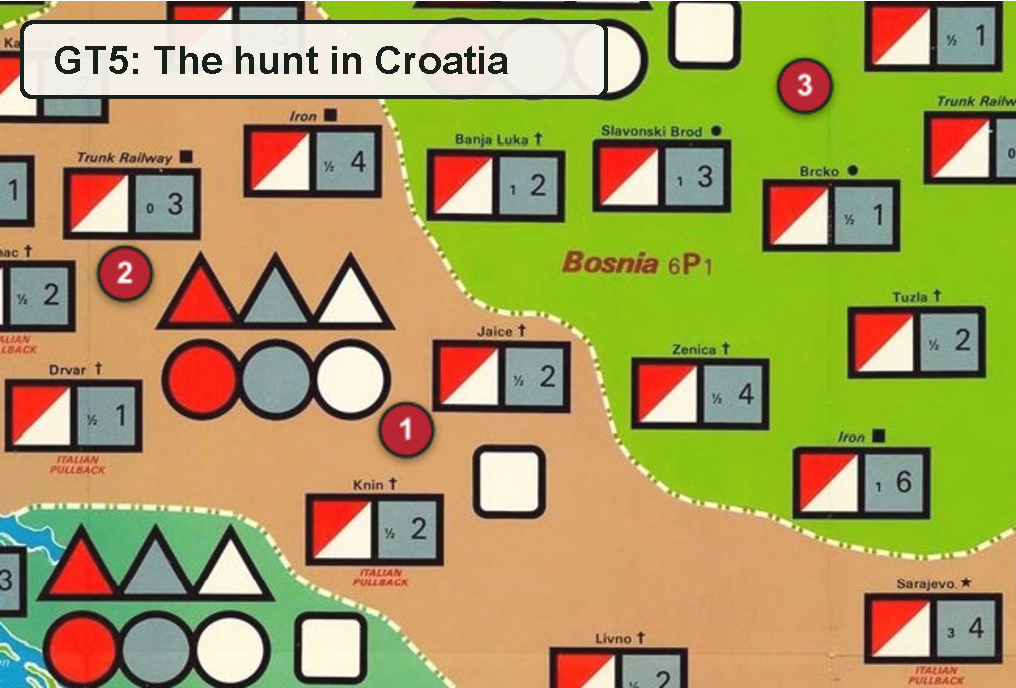
\includegraphics[height=2.42in,width=\linewidth,keepaspectratio]
    {playbook-turn-5-map.pdf}
  \mapcaption{Croatia and Bosnia: the hunt, AGO, and retreat}
\end{minipage}
\hfill
\begin{minipage}[t]{0.40\linewidth}
  \centering
  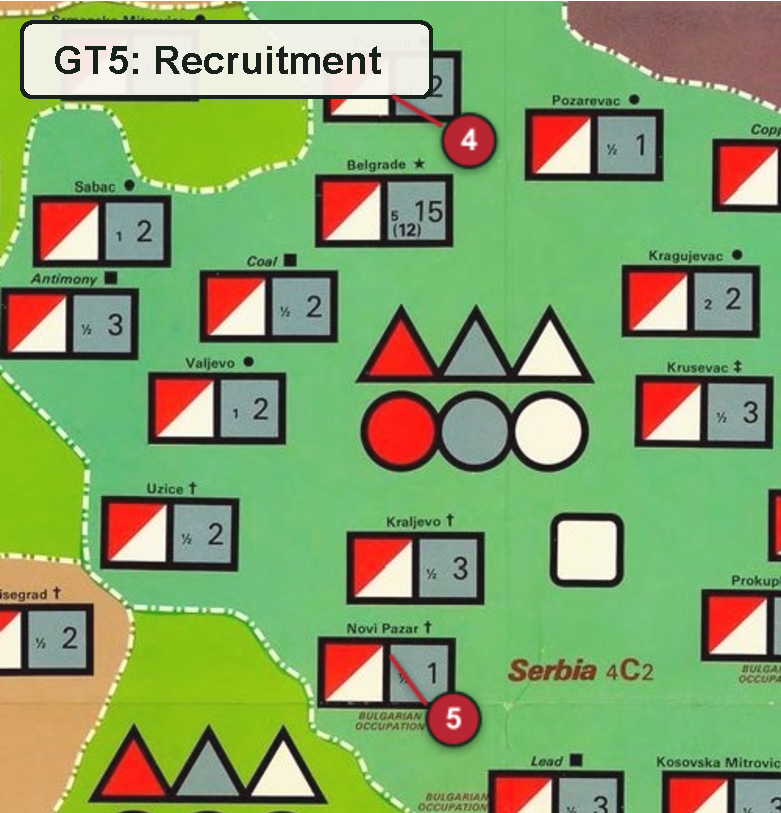
\includegraphics[height=2.42in,width=\linewidth,keepaspectratio]
    {playbook-turn-5-east-map.pdf}
  \mapcaption{Serbia: doubled recruitment penalty and one surviving source}
\end{minipage}
\end{center}

\begin{multicols}{2}
\small
\phase{A. Tito, Reinforcement, and Collaboration}

Tito was identified last turn, so the Axis may now attempt to locate him. The
roll is \die{6}: Tito is located~\mapbadge{1}, making the German 501st SS
Parachute Battalion available in the ensuing Axis Reinforcement Phase
\rulesref{9.42}. Place it in Croatia. Transfer German 342 as scheduled.

Resolve collaboration:

\begin{tabularx}{\linewidth}{@{}Xccc@{}}
  \toprule
  Stack & Roll & Mod. & Result \\
  \midrule
  Serbia neutral (2) & \die{5} & 0 & pro-Yugoslav \\
  Serbia pro-Yugoslav (1) & \die{2} & +1 & Neutral \\
  Montenegro pro-Axis (4) & \die{3} & $-1$ & pro-Axis \\
  \bottomrule
\end{tabularx}

\phase{A. Anti-Guerrilla Operation: Croatia}

The Axis commits the 501st SS, German 704, Italian Bergamo, and two Croat
mountain brigades to the Croatia operation~\mapbadge{2}: 23 SP in all. The
Reaction roll is \die{1}. The Yugoslav Player moves an exposed Partisan group
elsewhere but deliberately leaves Tito and both Partisan brigades in the
Croatia Mountain so the tutorial can demonstrate the elimination procedure.

Deploy the entire Axis force in the corresponding Axis Mountain. Before normal
combat, make the one permitted elimination attempt \rulesref{9.43}. The Axis
rolls \die{3}; Tito is not eliminated, but is withdrawn for three full
Game-Turns. Put his counter aside. He will return as a Partisan reinforcement
on Game-Turn 9.

\begin{commentarybox}
The attempt has now been spent even though Tito survived. A result of 6 would
have eliminated him; 1--5 withdraws him for that many full Game-Turns.
\end{commentarybox}

\columnbreak

\textbf{Resolve the AGO combat.} The Partisan brigades defend with 8 SP.
Twenty-three to eight rounds down to 2:1; the AGO adjustment moves the attack
to 4:1. A \die{3} produces D1, doubled to D2. A strength-4 brigade cannot
satisfy a 2-SP loss, so no unit is eliminated, but both brigades must retreat.
The Axis chooses the Bosnia Partisan Hide-away~\mapbadge{3}
\rulesref{8.22A, 8.46}.

\phase{B--D. Player-Turns and Victory Points}

During Yugoslav Movement, move the two brigades from the Bosnia Hide-away to
the Bosnia Mountain. Move two groups from Novi Pazar to Pančevo, leaving seven
at Novi Pazar.

Victory Points:

\begin{tabularx}{\linewidth}{@{}Xr@{}}
  Pančevo, Novi Pazar, Tuzla, Cetinje & 6 \\
  Bosnia Mountain: 8 SP, 2 units & 2 \\
  Slovenia Mountain: 6 SP & 1 \\
  Tito withdrawn & $-5$ \\
  \midrule
  Turn total & 4 \\
\end{tabularx}

The running total is \textbf{24 VP}.

\phase{E. Terminal Stage}

Tito's absence halves all Objective and Mountain recruitment
\rulesref{9.32}. At drought-stricken Pančevo~\mapbadge{4}, recruitment would
be halved for drought and again for Tito's absence. More than one halving means
\textbf{no reinforcement} \rulesref{7.49}.

Elsewhere, Bosnia Mountain creates 1 group after Tito's modifier. Rolls of
\die{4} at Novi Pazar~\mapbadge{5} and \die{4} at Tuzla create 1 group apiece
after the same modifier. A \die{2} at Cetinje and the Slovenia Mountain
calculation both round to zero. The three available group counters are now all
in use.

Bosnia now has only three division equivalents against its Garrison Value of
6. An uprising roll of \die{2}, reduced by Bosnia's modifier of 1, would
generate three Partisan groups after an even alignment roll of \die{2}.
None can be placed because the Partisan group counter mix is exhausted
\rulesref{7.53, 7.68}.
\end{multicols}

\turnledger{+4}{24}{30 groups + 2 brigades}{2 / 4 / 1}{3 of 8}

\clearpage
\section{After Five Turns}

\begin{lessonbox}
The example stops at a natural transition point. The Partisans have organized
into brigades, German movement has expanded, the Chetniks are politically
fragmented, and Tito is temporarily off map. Game-Turn 6 will introduce Allied
Progress and a new Weather determination.
\end{lessonbox}

\begin{multicols}{2}
\small
\subsection{End Position}

\rowcolors{2}{TitoBlue!42}{white}
\begin{tabularx}{\linewidth}{@{}>{\bfseries}l X@{}}
  \rowcolor{TitoInk!15}
  Item & State after Game-Turn 5 \\
  Yugoslav VP & 24 \\
  Partisans & 30 groups, 2 brigades \\
  Tito & Withdrawn; returns GT9 \\
  Chetniks & 2 pro-Yugoslav, 4 pro-Axis, 1 neutral \\
  AGO reserve & 5 remain from the secret limit of 8 \\
  Weather & Drought ends with GT5 \\
  Brigade trigger & In effect since GT3 \\
  Bulgarian 25/27 & Deployed in Serbia \\
  German 342 & Transferred on GT5 \\
\end{tabularx}
\rowcolors{2}{}{}

\subsection{What Happens on Game-Turn 6?}

\begin{enumerate}[leftmargin=1.4em,itemsep=2pt]
  \item Begin Allied Progress in Box 1 and make the first progress roll
    \rulesref{10.11}.
  \item Make the GT6 Weather roll, establishing conditions through GT9
    \rulesref{11.22B}.
  \item Tito remains off map; skip identification and location.
  \item Deploy German 7SS \rulesref{13.91}.
  \item Continue collaboration and decide whether another AGO is worth one of
    the five remaining operations.
\end{enumerate}

\begin{commentarybox}[title={Do not read 24 VP as a forecast}]
The tutorial makes conservative Objective choices and deliberately exposes
Tito. Its running total exists to teach the Victory Point Stage, not to model
expert Yugoslav play or predict the final result.
\end{commentarybox}

\columnbreak

\subsection{Five Opening Lessons}

\begin{enumerate}[leftmargin=1.4em,itemsep=3pt]
  \item \textbf{Occupation is temporary.} Guerrillas can collect VP and
    recruits without defeating every Axis unit, but an Axis response can force
    them back into the Hide-aways.
  \item \textbf{The political map matters.} Chetnik allegiance changes can
    transfer whole stacks between players or remove them from both players'
    control.
  \item \textbf{Reaction is the defense against AGOs.} Moving Tito or an
    organized unit before deployment may matter more than preserving isolated
    groups.
  \item \textbf{Garrison arithmetic drives growth.} A large Zone shortfall can
    create more Partisans than routine Objective recruitment.
  \item \textbf{Triggers reshape the war.} The first brigade widens German
    movement, releases Bulgarian reinforcements, and starts the hunt for Tito.
\end{enumerate}

\subsection{Rules Used Most Often}

\begin{tabularx}{\linewidth}{@{}>{\bfseries}l X@{}}
  4.2 & Sequence of Play \\
  6.1--6.4 & Movement and stacking \\
  7.2 & Chetnik collaboration \\
  7.4--7.6 & Recruitment, uprisings, organization \\
  8.1--8.3 & Combat and terrain \\
  8.4 & Anti-Guerrilla Operations \\
  9.3--9.4 & Tito, recruitment, and the hunt \\
  11.0 & Weather \\
  13.9 & Reinforcement and transfer schedule \\
  14.2--14.3 & Victory Points \\
\end{tabularx}
\end{multicols}

\vfill
{\color{TitoInk}\hrule height 0.7pt}
\vspace{5pt}
\begin{center}
  {\sffamily\bfseries\large Continue the game from Game-Turn 6—or reset the
  pieces and try a different opening.\par}
  \vspace{5pt}
  \counterpic[0.58in]{tito-identified}\hspace{0.14in}
  \counterpic[0.58in]{partisan-brigade}\hspace{0.14in}
  \counterpic[0.58in]{german-parachute}\hspace{0.14in}
  \counterpic[0.58in]{anti-guerrilla-operations}
\end{center}


\end{document}
